\section{Roteiro Prático 05 (Parte 2) — Tarefa Guiada: Refatoração da Vitrine de Serviços (Flask \& SQLite)}

% =====================================================
% OBJETIVOS DA ATIVIDADE GUIADA
% =====================================================

\begin{boxObjetivos}[Objetivos de Aprendizagem — Roteiro 05 (Parte 2: Tarefa Guiada)]
\textbf{Objetivos da Tarefa Prática (Refatoração Arquitetural da Vitrine de Serviços)}

Ao longo desta tarefa de implementação orientada passo a passo, o estudante irá:

\begin{itemize}[leftmargin=*]
\item Desenvolver e estruturar o backend RESTful em \textbf{Python Flask} com suporte a CORS para fornecer endpoints de consulta (\texttt{GET /api/servicos}) e cadastro (\texttt{POST /api/servicos});
\item Configurar a persistência relacional com \textbf{SQLite 3} em arquivo físico (\texttt{vitrine.db}), aplicando comandos SQL de criação de tabelas e inserção parametrizada para prevenir injeção de SQL;
\item Refatorar o módulo de serviços do frontend (\texttt{vitrineService.js}) com a moderna \textbf{Fetch API} (\texttt{async/await}), substituindo o acesso síncrono ao \texttt{localStorage};
\item Implementar o padrão profissional de \textbf{Contingência Resiliente (Fallback)}: se a API do Flask responder, a aplicação consome o banco de dados; caso o servidor caia ou a página rode no GitHub Pages, os dados são lidos/gravados no \texttt{localStorage} em modo de cache de segurança;
\item Enriquecer a camada de visualização (\texttt{vitrineView.js}) com \textbf{Spinners de Carregamento} reativos e \textbf{Badges dinâmicos de conectividade} com a API (\textit{"Conectado à API (SQLite)"} vs \textit{"Modo Offline (LocalStorage)"});
\item Adaptar o controlador orquestrador (\texttt{main.js}) para lidar com promessas assíncronas no carregamento e na submissão do formulário modal;
\item Executar baterias de testes práticos de integração e validar a resiliência contra quedas propositais do servidor.
\end{itemize}
\end{boxObjetivos}

\begin{figure}[H]
    \centering
    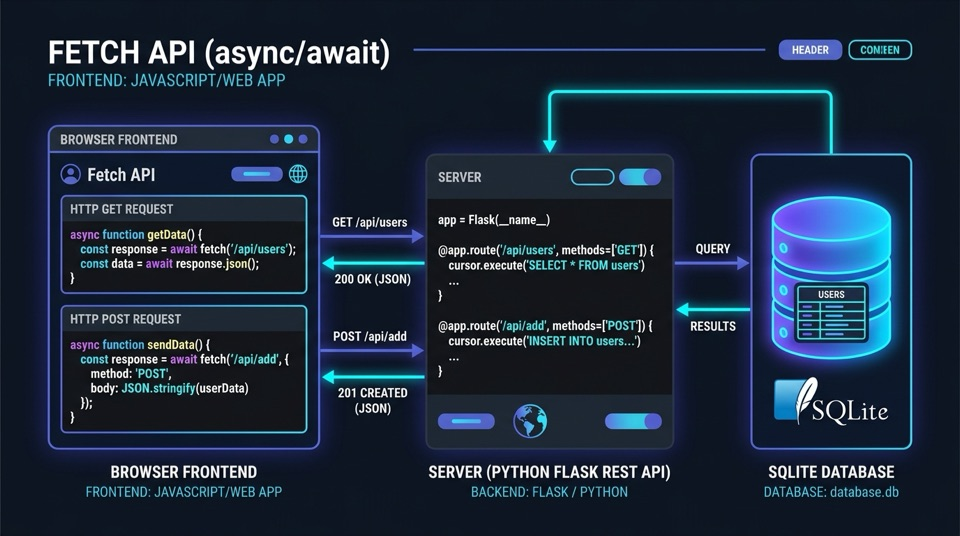
\includegraphics[width=0.88\textwidth]{roteiro5_fetch_api.jpg}
    \caption{Visão Geral da Aplicação Integrada: Vitrine de Serviços conectada via Fetch API com backend Flask, SQLite persistente e contingência offline.}
    \label{fig:preview_roteiro5_parte2}
\end{figure}

\subsection{Estrutura do Projeto Integrado (\texttt{exercicio-roteiro5/})}

Para esta tarefa de refatoração, o projeto está estruturado de forma desacoplada entre cliente (\textit{frontend}) e servidor (\textit{backend}):

\begin{boxCodigoTerminal}
\fontsize{8.5pt}{11pt}\selectfont
\begin{verbatim}
roteiro-5/
|-- exercicio-roteiro5/
    |-- backend/
    |   |-- app.py                # Servidor Flask com rotas REST e SQLite
    |   |-- requirements.txt      # Dependências (Flask, Flask-CORS)
    |   \-- vitrine.db            # Banco SQLite (gerado automaticamente)
    |-- css/
    |   \-- styles.css            # Estilos customizados e animações
    |-- js/
    |   |-- services/
    |   |   \-- vitrineService.js # Camada de dados assíncrona (Fetch + Fallback)
    |   |-- views/
    |   |   \-- vitrineView.js    # Renderização DOM (cards, spinners, badges)
    |   |-- utils/
    |   |   \-- formatters.js     # Funções utilitárias puras
    |   \-- main.js               # Orquestrador assíncrono e eventos
    \-- index.html                # Interface HTML5 + Bootstrap 5 + Modal
\end{verbatim}
\end{boxCodigoTerminal}

% FASES DE IMPLEMENTAÇÃO GUIADAS (ZERO-ELLIPSIS RULE)
% =====================================================

\newpage
\subsection{Implementação Passo a Passo Guiada}

Seguiremos a sequência didática em 6 fases de implementação estruturadas. Todo o código fornecido é **100\% completo, sem reticências ou omissões**.

% --- FASE 1 ---
\begin{boxAtividade}[{Fase 1/6: Configuração do Backend em Flask \& SQLite (backend/)}]
\textbf{Responsabilidade Arquitetural:} Criar o ambiente isolado Python (virtualenv), instalar o microframework Flask com suporte a CORS e implementar a API RESTful com conexão ao SQLite em arquivo (\texttt{vitrine.db}).
\end{boxAtividade}

\textbf{Passo 1.1: Criar o arquivo de dependências (\texttt{backend/requirements.txt})}
\begin{boxCodigoTerminal}
\fontsize{8.5pt}{11pt}\selectfont
\begin{verbatim}
Flask>=3.0.0
flask-cors>=4.0.0
\end{verbatim}
\end{boxCodigoTerminal}

\textbf{Passo 1.2: No terminal do VS Code, criar o ambiente virtual e instalar dependências:}
\begin{boxCodigoTerminal}
\fontsize{8.5pt}{11pt}\selectfont
\begin{verbatim}
# Acesse a pasta do backend
cd roteiro-5/exercicio-roteiro5/backend

# Cria o ambiente virtual isolado
python3 -m venv venv

# Ativa o ambiente virtual (Linux/Mac)
source venv/bin/activate
# No Windows PowerShell utilize: .\venv\Scripts\Activate.ps1

# Instala o Flask e o CORS
pip install -r requirements.txt
\end{verbatim}
\end{boxCodigoTerminal}

\textbf{Passo 1.3: Criar o arquivo completo do servidor (\texttt{backend/app.py}):}
\begin{boxCodigoPY}
import os
import sqlite3
from datetime import datetime
from flask import Flask, jsonify, request
from flask_cors import CORS

app = Flask(__name__)
# Habilita CORS para permitir que o Live Server (porta 5500) acesse o Flask (5000)
CORS(app)

DB_PATH = os.path.join(os.path.dirname(__file__), 'vitrine.db')

def obter_conexao():
    """Conecta ao SQLite retornando linhas como dicionários."""
    conn = sqlite3.connect(DB_PATH)
    conn.row_factory = sqlite3.Row
    return conn

def inicializar_banco():
    """Cria a tabela servicos e popula com os 3 registros modelo de Garopaba se vazia."""
    conn = obter_conexao()
    cursor = conn.cursor()
    cursor.execute('''
        CREATE TABLE IF NOT EXISTS servicos (
            id INTEGER PRIMARY KEY AUTOINCREMENT,
            nome TEXT NOT NULL,
            categoria TEXT NOT NULL,
            bairro TEXT NOT NULL,
            precoBase REAL NOT NULL,
            telefone TEXT NOT NULL,
            descricao TEXT,
            dataCadastro TEXT
        )
    ''')

    cursor.execute('SELECT COUNT(*) AS total FROM servicos')
    if cursor.fetchone()['total'] == 0:
        dados_semente = [
            (
                'Maré Alta Artesanatos & Cerâmicas', 'Artesanato', 'Centro Histórico',
                35.00, '48991234567',
                'Peças artesanais e utilitárias modeladas à mão com argila local e conchas de Garopaba.',
                datetime.now().isoformat()
            ),
            (
                'Garopaba Web & Design Studio', 'Tecnologia', 'Ferrugem',
                150.00, '48998765432',
                'Criação de websites profissionais responsivos, cardápios digitais e suporte para comércio local.',
                datetime.now().isoformat()
            ),
            (
                'Pescado Fresco do Zequinha', 'Alimentação', 'Canto das Canoas',
                42.00, '48984561234',
                'Peixes frescos e frutos do mar da pesca artesanal diária entregues com higiene e pontualidade.',
                datetime.now().isoformat()
            )
        ]
        cursor.executemany('''
            INSERT INTO servicos (nome, categoria, bairro, precoBase, telefone, descricao, dataCadastro)
            VALUES (?, ?, ?, ?, ?, ?, ?)
        ''', dados_semente)
        conn.commit()
    conn.close()

@app.route('/api/status', methods=['GET'])
def verificar_status():
    """Diagnóstico de conectividade com a API."""
    return jsonify({
        'status': 'online',
        'mensagem': 'API REST da Vitrine de Garopaba operacional.',
        'banco': 'SQLite 3'
    }), 200

@app.route('/api/servicos', methods=['GET'])
def listar_servicos():
    """READ: Retorna a lista de todos os serviços ordenados pelo ID decrescente."""
    conn = obter_conexao()
    cursor = conn.cursor()
    cursor.execute('SELECT * FROM servicos ORDER BY id DESC')
    linhas = cursor.fetchall()
    conn.close()
    return jsonify([dict(l) for l in linhas]), 200

@app.route('/api/servicos', methods=['POST'])
def cadastrar_servico():
    """CREATE: Grava um novo serviço enviado em formato JSON no SQLite."""
    dados = request.get_json()
    if not dados:
        return jsonify({'erro': 'Payload inválido.'}), 400

    conn = obter_conexao()
    cursor = conn.cursor()
    data_atual = datetime.now().isoformat()

    cursor.execute('''
        INSERT INTO servicos (nome, categoria, bairro, precoBase, telefone, descricao, dataCadastro)
        VALUES (?, ?, ?, ?, ?, ?, ?)
    ''', (
        dados['nome'].strip(),
        dados['categoria'].strip(),
        dados['bairro'].strip(),
        float(dados['precoBase']),
        dados['telefone'].strip(),
        dados.get('descricao', '').strip(),
        data_atual
    ))
    conn.commit()
    novo_id = cursor.lastrowid
    conn.close()

    return jsonify({
        'id': novo_id,
        'nome': dados['nome'].strip(),
        'categoria': dados['categoria'].strip(),
        'bairro': dados['bairro'].strip(),
        'precoBase': float(dados['precoBase']),
        'telefone': dados['telefone'].strip(),
        'descricao': dados.get('descricao', '').strip(),
        'dataCadastro': data_atual
    }), 201

@app.route('/api/servicos/<int:id>', methods=['DELETE'])
def excluir_servico(id):
    """DELETE: Exclui um serviço pelo ID."""
    conn = obter_conexao()
    cursor = conn.cursor()
    cursor.execute('DELETE FROM servicos WHERE id = ?', (id,))
    conn.commit()
    conn.close()
    return jsonify({'mensagem': f'Serviço {id} removido.'}), 200

if __name__ == '__main__':
    inicializar_banco()
    print('Servidor Flask ativo na porta 5000: http://127.0.0.1:5000')
    app.run(host='127.0.0.1', port=5000, debug=True)
\end{boxCodigoPY}

% --- FASE 2 ---
\newpage
\begin{boxAtividade}[{Fase 2/6: Executando e Testando a API RESTful}]
\textbf{Responsabilidade Arquitetural:} Iniciar o servidor Flask na porta 5000 e validar os endpoints de saúde (\texttt{/api/status}) e listagem (\texttt{/api/servicos}) diretamente no terminal e navegador antes da integração.
\end{boxAtividade}

\textbf{Passo 2.1: Iniciar o servidor no terminal:}
\begin{boxCodigoTerminal}
\fontsize{8.5pt}{11pt}\selectfont
\begin{verbatim}
python app.py
\end{verbatim}
\end{boxCodigoTerminal}

\textbf{Passo 2.2: Testar no navegador ou via cURL em outra aba do terminal:}
\begin{boxCodigoTerminal}
\fontsize{8.5pt}{11pt}\selectfont
\begin{verbatim}
curl http://127.0.0.1:5000/api/status
\end{verbatim}
\end{boxCodigoTerminal}

\textbf{Resposta esperada do servidor (JSON com status 200):}
\begin{boxCodigoTerminal}
\fontsize{8.5pt}{11pt}\selectfont
\begin{verbatim}
{"banco":"SQLite 3","mensagem":"API REST da Vitrine de Garopaba operacional.","status":"online"}
\end{verbatim}
\end{boxCodigoTerminal}

\begin{boxTeste}{Checkpoint de Validação da Fase 2}
Abra no navegador \url{http://127.0.0.1:5000/api/servicos}. Você deverá ver a lista JSON com os 3 registros semente cadastrados automaticamente no arquivo \texttt{vitrine.db}.
\end{boxTeste}

% --- FASE 3 ---
\begin{boxAtividade}[{Fase 3/6: A Revolução Assíncrona no vitrineService.js}]
\textbf{Responsabilidade Arquitetural:} Refatorar os métodos de leitura e escrita para utilizarem requisições HTTP assíncronas com \texttt{fetch()} e \texttt{async/await}, mantendo uma camada de contingência transparente com \texttt{localStorage}.
\end{boxAtividade}

\begin{boxCodigoJS}
// js/services/vitrineService.js
const API_BASE_URL = 'http://127.0.0.1:5000/api';
const STORAGE_KEY = 'garopaba_vitrine_servicos';

let apiConectada = false;

export const DADOS_INICIAIS = [
  {
    id: '1',
    nome: 'Maré Alta Artesanatos & Cerâmicas',
    categoria: 'Artesanato',
    bairro: 'Centro Histórico',
    precoBase: 35.00,
    telefone: '48991234567',
    descricao: 'Peças artesanais e utilitárias modeladas à mão com argila local e conchas de Garopaba.'
  },
  {
    id: '2',
    nome: 'Garopaba Web & Design Studio',
    categoria: 'Tecnologia',
    bairro: 'Ferrugem',
    precoBase: 150.00,
    telefone: '48998765432',
    descricao: 'Criação de websites profissionais responsivos, cardápios digitais e suporte para comércio local.'
  },
  {
    id: '3',
    nome: 'Pescado Fresco do Zequinha',
    categoria: 'Alimentação',
    bairro: 'Canto das Canoas',
    precoBase: 42.00,
    telefone: '48984561234',
    descricao: 'Peixes frescos e frutos do mar da pesca artesanal diária entregues com higiene e pontualidade.'
  }
];

export function estaConectadoNaApi() {
  return apiConectada;
}

export async function testarConexaoApi() {
  try {
    const resposta = await fetch(`${API_BASE_URL}/status`, {
      method: 'GET',
      headers: { 'Accept': 'application/json' },
      signal: AbortSignal.timeout(2000)
    });
    apiConectada = resposta.ok;
    return apiConectada;
  } catch (erro) {
    apiConectada = false;
    return false;
  }
}

// Rotinas Locais de Contingência (Fallback)
function obterServicosLocal() {
  const dados = localStorage.getItem(STORAGE_KEY);
  if (!dados) {
    localStorage.setItem(STORAGE_KEY, JSON.stringify(DADOS_INICIAIS));
    return DADOS_INICIAIS;
  }
  try { return JSON.parse(dados); } catch (e) { return []; }
}

function salvarServicoLocal(novoServico) {
  const servicos = obterServicosLocal();
  const servicoCompleto = {
    id: Date.now().toString(),
    dataCadastro: new Date().toISOString(),
    ...novoServico
  };
  servicos.unshift(servicoCompleto);
  localStorage.setItem(STORAGE_KEY, JSON.stringify(servicos));
  return servicoCompleto;
}

function removerServicoLocal(id) {
  const servicos = obterServicosLocal();
  const filtrados = servicos.filter(s => s.id.toString() !== id.toString());
  localStorage.setItem(STORAGE_KEY, JSON.stringify(filtrados));
  return filtrados;
}

// Operações Assíncronas com Fetch API
export async function obterServicos() {
  try {
    const resposta = await fetch(`${API_BASE_URL}/servicos`, {
      method: 'GET',
      headers: { 'Accept': 'application/json' },
      signal: AbortSignal.timeout(3000)
    });
    if (!resposta.ok) throw new Error(`HTTP ${resposta.status}`);
    const dados = await resposta.json();
    apiConectada = true;
    localStorage.setItem(STORAGE_KEY, JSON.stringify(dados));
    return dados;
  } catch (erro) {
    apiConectada = false;
    console.warn('API Flask offline. Ativando contingência LocalStorage:', erro.message);
    return obterServicosLocal();
  }
}

export async function salvarServico(novoServico) {
  try {
    const resposta = await fetch(`${API_BASE_URL}/servicos`, {
      method: 'POST',
      headers: {
        'Content-Type': 'application/json',
        'Accept': 'application/json'
      },
      body: JSON.stringify(novoServico),
      signal: AbortSignal.timeout(4000)
    });
    if (!resposta.ok) throw new Error(`HTTP ${resposta.status}`);
    const criado = await resposta.json();
    apiConectada = true;
    const servicos = obterServicosLocal();
    servicos.unshift(criado);
    localStorage.setItem(STORAGE_KEY, JSON.stringify(servicos));
    return criado;
  } catch (erro) {
    apiConectada = false;
    console.warn('Falha no envio à API. Salvando localmente:', erro.message);
    return salvarServicoLocal(novoServico);
  }
}

export async function removerServico(id) {
  try {
    const resposta = await fetch(`${API_BASE_URL}/servicos/${id}`, {
      method: 'DELETE',
      headers: { 'Accept': 'application/json' },
      signal: AbortSignal.timeout(4000)
    });
    if (!resposta.ok) throw new Error(`HTTP ${resposta.status}`);
    apiConectada = true;
    removerServicoLocal(id);
    return true;
  } catch (erro) {
    apiConectada = false;
    console.warn('Falha na exclusão remota. Removendo localmente:', erro.message);
    removerServicoLocal(id);
    return true;
  }
}
\end{boxCodigoJS}

% --- FASE 4 ---
\newpage
\begin{boxAtividade}[{Fase 4/6: Camada de Visão \& Feedbacks de Rede (vitrineView.js)}]
\textbf{Responsabilidade Arquitetural:} Adicionar componentes visuais de carregamento (\texttt{exibirSpinner}) e indicador de conectividade em tempo real com a API no topo da página.
\end{boxAtividade}

\begin{boxCodigoJS}
// js/views/vitrineView.js
import { formatarMoeda, formatarTelefone, escapeHtml } from '../utils/formatters.js';

const CORES_CATEGORIA = {
  'Alimentação': 'success',
  'Tecnologia': 'info',
  'Artesanato': 'warning',
  'Serviços Gerais': 'primary',
  'Turismo': 'secondary'
};

export function criarCardHtml(s) {
  const corBadge = CORES_CATEGORIA[s.categoria] || 'primary';
  const telNumeros = (s.telefone || '').replace(/\D/g, '');

  return `
    <div class="col-md-6 col-lg-4 mb-4">
      <div class="card h-100 shadow-sm border-0 vitrine-card rounded-4 overflow-hidden">
        <div class="card-body p-4 d-flex flex-column">
          <div class="d-flex justify-content-between align-items-center mb-2">
            <span class="badge bg-${corBadge} px-3 py-2 rounded-pill font-outfit">
              <i class="bi bi-tag-fill me-1"></i>${escapeHtml(s.categoria)}
            </span>
            <span class="fw-bold text-success font-outfit fs-5">
              ${formatarMoeda(s.precoBase)}
            </span>
          </div>

          <h5 class="card-title fw-bold text-dark mt-2 mb-1">${escapeHtml(s.nome)}</h5>
          <h6 class="text-muted small mb-3">
            <i class="bi bi-geo-alt-fill text-danger me-1"></i>${escapeHtml(s.bairro)}
          </h6>
          <p class="card-text text-secondary small flex-grow-1" style="line-height: 1.5;">
            ${escapeHtml(s.descricao)}
          </p>

          <hr class="my-3 text-muted opacity-25">

          <div class="d-flex justify-content-between align-items-center mt-auto">
            <a href="https://wa.me/55${telNumeros}" target="_blank" class="btn btn-sm btn-outline-success rounded-pill px-3 fw-bold">
              <i class="bi bi-whatsapp me-1"></i>${formatarTelefone(s.telefone)}
            </a>
            <div class="d-flex gap-1">
              <button class="btn btn-sm btn-outline-danger btn-excluir rounded-pill px-2" data-id="${s.id}" title="Remover da vitrine">
                <i class="bi bi-trash"></i>
              </button>
            </div>
          </div>
        </div>
      </div>
    </div>
  `;
}

export function renderizarCards(servicos, containerElement) {
  if (!containerElement) return;
  if (!servicos || servicos.length === 0) {
    containerElement.innerHTML = `
      <div class="col-12 py-5 text-center text-muted">
        <i class="bi bi-inbox fs-1 d-block mb-3 text-secondary opacity-50"></i>
        <h5 class="fw-bold">Nenhum serviço encontrado</h5>
        <p class="small">Cadastre um novo serviço ou altere o filtro de categoria.</p>
      </div>
    `;
    return;
  }
  containerElement.innerHTML = servicos.map(s => criarCardHtml(s)).join('');
}

export function exibirSpinner(containerElement) {
  if (!containerElement) return;
  containerElement.innerHTML = `
    <div class="col-12 py-5 text-center text-primary">
      <div class="spinner-border text-primary" role="status" style="width: 3rem; height: 3rem;">
        <span class="visually-hidden">Carregando dados da API...</span>
      </div>
      <p class="mt-3 text-muted small fw-semibold">Consultando serviços no backend Flask (SQLite)...</p>
    </div>
  `;
}

export function atualizarStatusConexao(isOnline, statusBadgeEl) {
  if (!statusBadgeEl) return;
  if (isOnline) {
    statusBadgeEl.className = 'badge bg-success-subtle text-success border border-success-subtle px-3 py-2 rounded-pill fw-semibold';
    statusBadgeEl.innerHTML = '<i class="bi bi-cloud-check-fill me-1"></i> Backend Online (Flask + SQLite)';
  } else {
    statusBadgeEl.className = 'badge bg-warning-subtle text-warning border border-warning-subtle px-3 py-2 rounded-pill fw-semibold';
    statusBadgeEl.innerHTML = '<i class="bi bi-hdd-network-fill me-1"></i> Modo Offline (LocalStorage)';
  }
}

export function exibirToast(mensagem, tipo = 'success') {
  const toastEl = document.getElementById('toastNotificacao');
  const toastMsgEl = document.getElementById('toastMensagem');
  if (!toastEl || !toastMsgEl) return;
  toastEl.className = `toast align-items-center text-white bg-${tipo} border-0 shadow-lg`;
  toastMsgEl.innerText = mensagem;
  const bsToast = bootstrap.Toast.getOrCreateInstance(toastEl, { delay: 3500 });
  bsToast.show();
}
\end{boxCodigoJS}

% --- FASE 5 ---
\newpage
\begin{boxAtividade}[{Fase 5/6: Orquestrador Assíncrono da Aplicação (main.js)}]
\textbf{Responsabilidade Arquitetural:} Coordenar os fluxos de eventos da interface utilizando \texttt{await} para aguardar a persistência no banco remoto antes de fechar modais e atualizar a vitrine.
\end{boxAtividade}

\begin{boxCodigoJS}
// js/main.js
import {
  obterServicos,
  salvarServico,
  removerServico,
  testarConexaoApi,
  estaConectadoNaApi
} from './services/vitrineService.js';

import {
  renderizarCards,
  exibirSpinner,
  atualizarStatusConexao,
  exibirToast
} from './views/vitrineView.js';

document.addEventListener('DOMContentLoaded', async () => {
  const form = document.getElementById('formCadastro');
  const container = document.getElementById('vitrineContainer');
  const filtroCategoria = document.getElementById('filtroCategoria');
  const contadorEl = document.getElementById('totalServicosBadge');
  const statusApiBadge = document.getElementById('statusApiBadge');
  const modalEl = document.getElementById('modalCadastro');
  const btnSalvarTexto = document.getElementById('btnSalvarTexto');
  const btnSalvar = document.getElementById('btnSalvar');

  let cacheServicosAtuais = [];

  async function atualizarInterface() {
    exibirSpinner(container);
    const conectado = await testarConexaoApi();
    atualizarStatusConexao(conectado, statusApiBadge);

    cacheServicosAtuais = await obterServicos();
    const categoriaSelecionada = filtroCategoria ? filtroCategoria.value : 'todas';
    const servicosFiltrados = categoriaSelecionada === 'todas'
      ? cacheServicosAtuais
      : cacheServicosAtuais.filter(s => s.categoria === categoriaSelecionada);

    renderizarCards(servicosFiltrados, container);
    if (contadorEl) {
      contadorEl.innerText = `${cacheServicosAtuais.length} Serviços Cadastrados`;
    }
  }

  if (filtroCategoria) {
    filtroCategoria.addEventListener('change', () => {
      const categoria = filtroCategoria.value;
      const filtrados = categoria === 'todas'
        ? cacheServicosAtuais
        : cacheServicosAtuais.filter(s => s.categoria === categoria);
      renderizarCards(filtrados, container);
    });
  }

  // Inicialização assíncrona
  await atualizarInterface();

  // Reset do formulário ao abrir modal
  if (modalEl) {
    modalEl.addEventListener('show.bs.modal', () => {
      form.reset();
      form.classList.remove('was-validated');
    });
  }

  function obterValorCampo(idCampo) {
    const elemento = document.getElementById(idCampo);
    if (elemento) {
      return elemento.value.trim();
    }
    return '';
  }

  // Cadastro de Novo Serviço via HTTP POST (Função Nomeada)
  async function cadastrarNovoServico(evento) {
    evento.preventDefault();
    if (form.checkValidity() === false) {
      evento.stopPropagation();
      form.classList.add('was-validated');
      return;
    }

    const dados = {
      nome: obterValorCampo('nome'),
      categoria: document.getElementById('categoria').value,
      bairro: obterValorCampo('bairro'),
      precoBase: parseFloat(obterValorCampo('precoBase')) || 0,
      telefone: obterValorCampo('telefone'),
      descricao: obterValorCampo('descricao')
    };

    if (btnSalvar) btnSalvar.disabled = true;
    if (btnSalvarTexto) btnSalvarTexto.innerText = 'Gravando...';

    try {
      await salvarServico(dados);
      let msg = 'Serviço salvo localmente (Modo Offline).';
      if (estaConectadoNaApi() === true) {
        msg = 'Serviço gravado no banco de dados SQLite!';
      }
      exibirToast(msg, 'success');

      const modal = bootstrap.Modal.getOrCreateInstance(modalEl);
      modal.hide();
      await atualizarInterface();
    } catch (erro) {
      exibirToast('Erro ao processar cadastro.', 'danger');
    } finally {
      if (btnSalvar) btnSalvar.disabled = false;
      if (btnSalvarTexto) btnSalvarTexto.innerText = 'Salvar no Banco';
    }
  }

  form.addEventListener('submit', cadastrarNovoServico);

  // Exclusão Assíncrona via HTTP DELETE (Função Nomeada)
  async function tratarExclusaoNaVitrine(evento) {
    const btnExcluir = evento.target.closest('.btn-excluir');
    if (btnExcluir) {
      const id = btnExcluir.getAttribute('data-id');
      if (confirm('Deseja realmente remover este serviço da vitrine?')) {
        await removerServico(id);
        await atualizarInterface();
        exibirToast('Serviço excluído da vitrine.', 'warning');
      }
    }
  }

  container.addEventListener('click', tratarExclusaoNaVitrine);
});
\end{boxCodigoJS}

% --- FASE 6 ---
\newpage
\begin{boxAtividade}[{Fase 6/6: Verificação de Integração \& Prova de Contingência}]
\textbf{Responsabilidade Arquitetural:} Executar o roteiro de testes em dois cenários: com a API online no laboratório e com o servidor desligado comprovando a resiliência offline.
\end{boxAtividade}

\textbf{1. Teste Conectado (API Online):}
\begin{itemize}[leftmargin=*]
  \item Inicie o backend com \texttt{python app.py} na porta \texttt{5000};
  \item Abra o frontend via Live Server (\texttt{http://127.0.0.1:5500/index.html});
  \item O badge no topo deve exibir: \textbf{\textit{Backend Online (Flask + SQLite)}};
  \item Cadastre um novo serviço e observe a requisição HTTP POST sendo logada no terminal do Flask!
\end{itemize}

\textbf{2. Teste de Resiliência (Fallback LocalStorage):}
\begin{itemize}[leftmargin=*]
  \item No terminal do Flask, pressione \texttt{Ctrl + C} para desligar o servidor;
  \item Recarregue a página no navegador com \texttt{F5};
  \item O frontend detecta a indisponibilidade e muda o badge para: \textbf{\textit{Modo Offline (LocalStorage)}};
  \item Os cards continuam aparecendo normalmente a partir da cópia em cache!
\end{itemize}

\begin{boxTeste}{Critério de Conclusão da Tarefa Principal}
A aplicação demonstrou sucesso na comunicação assíncrona cliente-servidor via Fetch API, realizou persistência no SQLite e provou resiliência arquitetural ao operar em modo de contingência offline.
\end{boxTeste}

% =====================================================
% SEÇÃO DE MINI DESAFIOS PRÁTICOS (AUTONOMIA DO ESTUDANTE)
% =====================================================

\newpage
\subsection{Mini Desafios Práticos de Extensão \& Fixação}

Agora que sua arquitetura full-stack está completamente funcional e resiliente, propomos \textbf{3 mini desafios progressivos} para você consolidar como novas funcionalidades trafegam por todas as camadas do sistema (Banco SQLite $\rightarrow$ Backend Flask $\rightarrow$ Frontend JavaScript $\rightarrow$ Interface HTML5/Bootstrap).

\begin{boxDica}[Metodologia de Aprendizagem Ativa]
Recomendamos fortemente que você tente implementar cada um dos 3 desafios por conta própria no código do projeto antes de consultar o gabarito! Observe quais arquivos precisam ser ajustados e teste os resultados no navegador.
\end{boxDica}

\subsubsection*{Mini Desafio 1: Adicionar o Campo Booleano ``Aceita PIX''}
\textbf{Contexto:} Os comerciantes locais solicitaram que a vitrine indique claramente se o estabelecimento aceita pagamentos instantâneos via PIX.
\begin{itemize}[leftmargin=*]
  \item \textbf{No Banco SQLite e Backend (\texttt{backend/app.py}):} Adicionar a coluna \texttt{aceitaPix INTEGER DEFAULT 1} na tabela \texttt{servicos}. Na rota \texttt{POST /api/servicos}, capturar o booleano enviado no JSON e salvá-lo como \texttt{1} ou \texttt{0};
  \item \textbf{No Formulário Modal (\texttt{index.html}):} Inserir um interruptor (\textit{switch}) do Bootstrap com o identificador \texttt{id="aceitaPix"}, marcado como ativo por padrão (\texttt{checked});
  \item \textbf{No Orquestrador (\texttt{js/main.js}):} Coletar o valor booleano com \texttt{document.getElementById('aceitaPix').checked} e incluí-lo no objeto enviado ao backend;
  \item \textbf{Na Camada de Visão (\texttt{js/views/vitrineView.js}):} Se \texttt{s.aceitaPix} for verdadeiro, renderizar um badge verde elegante ao lado do badge de categoria no topo do card.
\end{itemize}

\subsubsection*{Mini Desafio 2: Contador Reativo de Serviços Cadastrados}
\textbf{Contexto:} A interface atual lista os serviços, mas os usuários não conseguem visualizar imediatamente quantos estabelecimentos estão cadastrados no total.
\begin{itemize}[leftmargin=*]
  \item \textbf{Na Interface (\texttt{index.html}):} Adicionar um badge de contador ao lado do subtítulo ou na barra de filtros com \texttt{id="totalServicosBadge"};
  \item \textbf{Na Camada de Visão (\texttt{js/views/vitrineView.js}):} Criar a função exportada \texttt{atualizarContadorServicos(total, elemento)} que exiba o texto no singular (\textit{"1 serviço cadastrado"}) ou no plural (\textit{"N serviços cadastrados"});
  \item \textbf{No Orquestrador (\texttt{js/main.js}):} Invocar a atualização do contador sempre que a lista for carregada da API e também imediatamente após a exclusão de um registro.
\end{itemize}

\subsubsection*{Mini Desafio 3: Campo de Seleção ``Prazo de Atendimento''}
\textbf{Contexto:} Diferentes serviços possuem prazos distintos (ex: pesca artesanal com entrega imediata vs estúdio de design sob agendamento prévio).
\begin{itemize}[leftmargin=*]
  \item \textbf{No Banco e Backend (\texttt{backend/app.py}):} Adicionar a coluna \texttt{prazoAtendimento TEXT DEFAULT 'Sob agendamento'} na tabela \texttt{servicos} e persistir o valor recebido no \texttt{POST};
  \item \textbf{No Modal (\texttt{index.html}):} Adicionar um campo \texttt{select} com \texttt{id="prazoAtendimento"} oferecendo opções como \textit{"Atendimento Imediato"}, \textit{"Em até 24 horas"}, \textit{"2 a 5 dias úteis"} e \textit{"Sob agendamento"};
  \item \textbf{No Orquestrador (\texttt{js/main.js}):} Coletar o valor selecionado no formulário e adicioná-lo ao payload do cadastro;
  \item \textbf{Na Camada de Visão (\texttt{js/views/vitrineView.js}):} Exibir uma linha no corpo do card com o ícone de relógio informando o prazo de atendimento do profissional.
\end{itemize}

% =====================================================
% GABARITO COMENTADO DOS MINI DESAFIOS
% =====================================================

\newpage
\subsection{Gabarito Comentado dos Mini Desafios (Código Completo)}

Confira a seguir as soluções completas de cada desafio, organizadas por arquivo. Todas as instruções seguem o princípio de código 100\% aplicável (*Zero-Ellipsis Rule*).

\begin{boxAtividade}[{Solução do Mini Desafio 1: Campo Booleano ``Aceita PIX''}]
\textbf{Passo 1.1: No arquivo \texttt{backend/app.py}}, ajuste a criação da tabela e o endpoint de cadastro:
\end{boxAtividade}

\begin{boxCodigoPY}[]
# No método inicializar_banco(), adicione a coluna aceitaPix:
cursor.execute('''
    CREATE TABLE IF NOT EXISTS servicos (
        id INTEGER PRIMARY KEY AUTOINCREMENT,
        nome TEXT NOT NULL,
        categoria TEXT NOT NULL,
        bairro TEXT NOT NULL,
        precoBase REAL NOT NULL,
        telefone TEXT NOT NULL,
        descricao TEXT,
        dataCadastro TEXT,
        aceitaPix INTEGER DEFAULT 1
    )
''')

# No endpoint cadastrar_servico(), colete o valor booleano e converta para 1 ou 0:
@app.route('/api/servicos', methods=['POST'])
def cadastrar_servico():
    dados = request.get_json()
    if not dados:
        return jsonify({'erro': 'Payload inválido.'}), 400

    conn = obter_conexao()
    cursor = conn.cursor()
    data_atual = datetime.now().isoformat()
    aceita_pix = 1 if dados.get('aceitaPix', True) else 0

    cursor.execute('''
        INSERT INTO servicos (nome, categoria, bairro, precoBase, telefone, descricao, dataCadastro, aceitaPix)
        VALUES (?, ?, ?, ?, ?, ?, ?, ?)
    ''', (
        dados['nome'].strip(),
        dados['categoria'].strip(),
        dados['bairro'].strip(),
        float(dados['precoBase']),
        dados['telefone'].strip(),
        dados.get('descricao', '').strip(),
        data_atual,
        aceita_pix
    ))
    conn.commit()
    novo_id = cursor.lastrowid
    conn.close()

    return jsonify({
        'id': novo_id,
        'mensagem': 'Serviço cadastrado com sucesso!',
        'aceitaPix': bool(aceita_pix)
    }), 201
\end{boxCodigoPY}

\begin{boxAtividade}[{Passo 1.2: No arquivo \texttt{index.html}, adicione o Switch no Modal de Cadastro}]
Insira o controle logo abaixo do campo de Telefone (WhatsApp):
\end{boxAtividade}

\begin{boxCodigoHTML}[]
<div class="mb-3">
  <div class="form-check form-switch p-2 ps-5 bg-light rounded-3 border">
    <input class="form-check-input" type="checkbox" role="switch" id="aceitaPix" checked>
    <label class="form-check-label fw-semibold text-dark" for="aceitaPix">
      <i class="bi bi-qr-code text-success me-1"></i> Aceita pagamento instantâneo via PIX
    </label>
  </div>
</div>
\end{boxCodigoHTML}

\begin{boxAtividade}[{Passo 1.3: No arquivo \texttt{js/main.js}, colete o valor do checkbox}]
Na função de submissão do formulário (\texttt{cadastrarNovoServico}), adicione a propriedade \texttt{aceitaPix}:
\end{boxAtividade}

\begin{boxCodigoJS}[]
const dados = {
  nome: obterValorCampo('nome'),
  categoria: document.getElementById('categoria').value,
  bairro: obterValorCampo('bairro'),
  precoBase: parseFloat(obterValorCampo('precoBase')) || 0,
  telefone: obterValorCampo('telefone'),
  descricao: obterValorCampo('descricao'),
  aceitaPix: document.getElementById('aceitaPix').checked
};
\end{boxCodigoJS}

\begin{boxAtividade}[{Passo 1.4: No arquivo \texttt{js/views/vitrineView.js}, renderize o Badge no Card}]
Atualize a função \texttt{criarCardHtml(s)} para renderizar condicionalmente o badge do PIX:
\end{boxAtividade}

\begin{boxCodigoJS}[]
export function criarCardHtml(s) {
  const corBadge = CORES_CATEGORIA[s.categoria] || 'primary';
  const telNumeros = (s.telefone || '').replace(/\D/g, '');
  const badgePixHtml = (s.aceitaPix === 1 || s.aceitaPix === true)
    ? '<span class="badge bg-success-subtle text-success border border-success-subtle rounded-pill font-outfit px-2 py-1"><i class="bi bi-qr-code me-1"></i>PIX</span>'
    : '';

  return `
    <div class="col-md-6 col-lg-4 mb-4">
      <div class="card h-100 shadow-sm border-0 vitrine-card rounded-4 overflow-hidden">
        <div class="card-body p-4 d-flex flex-column">
          <div class="d-flex justify-content-between align-items-center mb-2">
            <div class="d-flex align-items-center gap-1">
              <span class="badge bg-${corBadge} px-3 py-2 rounded-pill font-outfit">
                <i class="bi bi-tag-fill me-1"></i>${escapeHtml(s.categoria)}
              </span>
              ${badgePixHtml}
            </div>
            <span class="fw-bold text-success font-outfit fs-5">
              ${formatarMoeda(s.precoBase)}
            </span>
          </div>

          <h5 class="card-title fw-bold text-dark mt-2 mb-1">${escapeHtml(s.nome)}</h5>
          <h6 class="text-muted small mb-3">
            <i class="bi bi-geo-alt-fill text-danger me-1"></i>${escapeHtml(s.bairro)}
          </h6>
          <p class="card-text text-secondary small flex-grow-1" style="line-height: 1.5;">
            ${escapeHtml(s.descricao)}
          </p>

          <hr class="my-3 text-muted opacity-25">

          <div class="d-flex justify-content-between align-items-center mt-auto">
            <a href="https://wa.me/55${telNumeros}" target="_blank" class="btn btn-sm btn-outline-success rounded-pill px-3 fw-bold">
              <i class="bi bi-whatsapp me-1"></i>${formatarTelefone(s.telefone)}
            </a>
            <div class="d-flex gap-1">
              <button class="btn btn-sm btn-outline-danger btn-excluir rounded-pill px-2" data-id="${s.id}" title="Remover da vitrine">
                <i class="bi bi-trash"></i>
              </button>
            </div>
          </div>
        </div>
      </div>
    </div>
  `;
}
\end{boxCodigoJS}

\newpage
\begin{boxAtividade}[{Solução do Mini Desafio 2: Contador Reativo de Serviços}]
\textbf{Passo 2.1: No arquivo \texttt{index.html}}, adicione o elemento badge no cabeçalho da página:
\end{boxAtividade}

\begin{boxCodigoHTML}[]
<div class="d-flex flex-wrap justify-content-between align-items-center gap-2 mb-4">
  <div>
    <h1 class="h3 mb-1 text-primary fw-bold">
      <i class="bi bi-shop me-2"></i>Vitrine de Serviços de Garopaba
    </h1>
    <p class="text-muted small mb-0">
      Mural comunitário de prestadores locais e comércio da região.
    </p>
  </div>
  <div class="d-flex align-items-center gap-2">
    <span id="totalServicosBadge" class="badge bg-primary-subtle text-primary border border-primary-subtle rounded-pill px-3 py-2 fw-semibold">
      <i class="bi bi-collection me-1"></i> Carregando...
    </span>
    <span id="statusConexao" class="badge bg-secondary-subtle text-secondary border px-3 py-2 rounded-pill fw-semibold">
      <i class="bi bi-arrow-repeat me-1"></i> Verificando conexão...
    </span>
  </div>
</div>
\end{boxCodigoHTML}

\begin{boxAtividade}[{Passo 2.2: No arquivo \texttt{js/views/vitrineView.js}, crie a função de contagem}]
Exporte a nova função utilitária de renderização de contadores:
\end{boxAtividade}

\begin{boxCodigoJS}[]
export function atualizarContadorServicos(total, elementoBadge) {
  if (!elementoBadge) return;
  const texto = total === 1 ? '1 serviço ativo' : `${total} serviços ativos`;
  elementoBadge.innerHTML = `<i class="bi bi-collection me-1"></i> ${texto}`;
}
\end{boxCodigoJS}

\begin{boxAtividade}[{Passo 2.3: No arquivo \texttt{js/main.js}, conecte a contagem ao fluxo}]
Importe \texttt{atualizarContadorServicos} e atualize nas rotinas de carregamento e filtragem:
\end{boxAtividade}

\begin{boxCodigoJS}[]
// 1. Atualize o cabeçalho de importações de ./views/vitrineView.js:
import {
  renderizarCards,
  exibirSpinner,
  atualizarStatusConexao,
  atualizarContadorServicos,
  exibirToast
} from './views/vitrineView.js';

// 2. Atualize a função de renderização da vitrine:
async function atualizarInterface() {
  exibirSpinner(container);
  const badgeTotal = document.getElementById('totalServicosBadge');

  try {
    const todosServicos = await obterServicos();
    const categoriaSelecionada = selectFiltro ? selectFiltro.value : 'todas';

    let servicosFiltrados = todosServicos;
    if (categoriaSelecionada !== 'todas') {
      servicosFiltrados = todosServicos.filter(s => s.categoria === categoriaSelecionada);
    }

    renderizarCards(servicosFiltrados, container);
    atualizarContadorServicos(servicosFiltrados.length, badgeTotal);
  } catch (erro) {
    exibirToast('Erro ao atualizar a vitrine de serviços.', 'danger');
  }
}
\end{boxCodigoJS}

\newpage
\begin{boxAtividade}[{Solução do Mini Desafio 3: Campo de Seleção ``Prazo de Atendimento''}]
\textbf{Passo 3.1: No arquivo \texttt{backend/app.py}}, inclua a coluna \texttt{prazoAtendimento}:
\end{boxAtividade}

\begin{boxCodigoPY}[]
# Na criação da tabela em inicializar_banco():
cursor.execute('''
    CREATE TABLE IF NOT EXISTS servicos (
        id INTEGER PRIMARY KEY AUTOINCREMENT,
        nome TEXT NOT NULL,
        categoria TEXT NOT NULL,
        bairro TEXT NOT NULL,
        precoBase REAL NOT NULL,
        telefone TEXT NOT NULL,
        descricao TEXT,
        dataCadastro TEXT,
        aceitaPix INTEGER DEFAULT 1,
        prazoAtendimento TEXT DEFAULT 'Sob agendamento'
    )
''')

# No endpoint cadastrar_servico(), colete prazoAtendimento com fallback seguro:
@app.route('/api/servicos', methods=['POST'])
def cadastrar_servico():
    dados = request.get_json()
    if not dados:
        return jsonify({'erro': 'Payload inválido.'}), 400

    conn = obter_conexao()
    cursor = conn.cursor()
    data_atual = datetime.now().isoformat()
    aceita_pix = 1 if dados.get('aceitaPix', True) else 0
    prazo = dados.get('prazoAtendimento', 'Sob agendamento').strip()

    cursor.execute('''
        INSERT INTO servicos (nome, categoria, bairro, precoBase, telefone, descricao, dataCadastro, aceitaPix, prazoAtendimento)
        VALUES (?, ?, ?, ?, ?, ?, ?, ?, ?)
    ''', (
        dados['nome'].strip(),
        dados['categoria'].strip(),
        dados['bairro'].strip(),
        float(dados['precoBase']),
        dados['telefone'].strip(),
        dados.get('descricao', '').strip(),
        data_atual,
        aceita_pix,
        prazo
    ))
    conn.commit()
    novo_id = cursor.lastrowid
    conn.close()

    return jsonify({'id': novo_id, 'mensagem': 'Serviço salvo!'}), 201
\end{boxCodigoPY}

\begin{boxAtividade}[{Passo 3.2: No arquivo \texttt{index.html}, adicione o Dropdown no Modal}]
Insira o campo de seleção de prazo no formulário de cadastro:
\end{boxAtividade}

\begin{boxCodigoHTML}[]
<div class="mb-3">
  <label for="prazoAtendimento" class="form-label fw-semibold text-secondary">
    <i class="bi bi-clock-history me-1 text-primary"></i> Prazo Estimado de Atendimento
  </label>
  <select class="form-select" id="prazoAtendimento" required>
    <option value="Atendimento Imediato">Atendimento Imediato</option>
    <option value="Em até 24 horas">Em até 24 horas</option>
    <option value="2 a 5 dias úteis">2 a 5 dias úteis</option>
    <option value="Sob agendamento" selected>Sob agendamento</option>
  </select>
</div>
\end{boxCodigoHTML}

\begin{boxAtividade}[{Passo 3.3: No arquivo \texttt{js/main.js}, colete o valor do campo}]
No manipulador de cadastro, acrescente a leitura do campo:
\end{boxAtividade}

\begin{boxCodigoJS}[]
const dados = {
  nome: obterValorCampo('nome'),
  categoria: document.getElementById('categoria').value,
  bairro: obterValorCampo('bairro'),
  precoBase: parseFloat(obterValorCampo('precoBase')) || 0,
  telefone: obterValorCampo('telefone'),
  descricao: obterValorCampo('descricao'),
  aceitaPix: document.getElementById('aceitaPix').checked,
  prazoAtendimento: document.getElementById('prazoAtendimento').value
};
\end{boxCodigoJS}

\begin{boxAtividade}[{Passo 3.4: No arquivo \texttt{js/views/vitrineView.js}, exiba o Prazo no Card}]
Atualize \texttt{criarCardHtml(s)} para exibir a linha de prazo de atendimento logo abaixo do bairro:
\end{boxAtividade}

\begin{boxCodigoJS}[]
export function criarCardHtml(s) {
  const corBadge = CORES_CATEGORIA[s.categoria] || 'primary';
  const telNumeros = (s.telefone || '').replace(/\D/g, '');
  const badgePixHtml = (s.aceitaPix === 1 || s.aceitaPix === true)
    ? '<span class="badge bg-success-subtle text-success border border-success-subtle rounded-pill font-outfit px-2 py-1"><i class="bi bi-qr-code me-1"></i>PIX</span>'
    : '';
  const prazoTexto = escapeHtml(s.prazoAtendimento || 'Sob agendamento');

  return `
    <div class="col-md-6 col-lg-4 mb-4">
      <div class="card h-100 shadow-sm border-0 vitrine-card rounded-4 overflow-hidden">
        <div class="card-body p-4 d-flex flex-column">
          <div class="d-flex justify-content-between align-items-center mb-2">
            <div class="d-flex align-items-center gap-1">
              <span class="badge bg-${corBadge} px-3 py-2 rounded-pill font-outfit">
                <i class="bi bi-tag-fill me-1"></i>${escapeHtml(s.categoria)}
              </span>
              ${badgePixHtml}
            </div>
            <span class="fw-bold text-success font-outfit fs-5">
              ${formatarMoeda(s.precoBase)}
            </span>
          </div>

          <h5 class="card-title fw-bold text-dark mt-2 mb-1">${escapeHtml(s.nome)}</h5>
          <h6 class="text-muted small mb-2">
            <i class="bi bi-geo-alt-fill text-danger me-1"></i>${escapeHtml(s.bairro)}
          </h6>
          <div class="text-secondary small mb-2">
            <i class="bi bi-clock-history text-primary me-1"></i><strong>Prazo:</strong> ${prazoTexto}
          </div>
          <p class="card-text text-secondary small flex-grow-1" style="line-height: 1.5;">
            ${escapeHtml(s.descricao)}
          </p>

          <hr class="my-3 text-muted opacity-25">

          <div class="d-flex justify-content-between align-items-center mt-auto">
            <a href="https://wa.me/55${telNumeros}" target="_blank" class="btn btn-sm btn-outline-success rounded-pill px-3 fw-bold">
              <i class="bi bi-whatsapp me-1"></i>${formatarTelefone(s.telefone)}
            </a>
            <div class="d-flex gap-1">
              <button class="btn btn-sm btn-outline-danger btn-excluir rounded-pill px-2" data-id="${s.id}" title="Remover da vitrine">
                <i class="bi bi-trash"></i>
              </button>
            </div>
          </div>
        </div>
      </div>
    </div>
  `;
}
\end{boxCodigoJS}

% =====================================================
% RESUMO DAS TRANSFORMAÇÕES (O QUE MUDOU E POR QUE MUDOU)
% =====================================================

\newpage
\subsection{Quadro Comparativo: Evolução do Roteiro 04 para o Roteiro 05}

\begin{table}[H]
\centering
\small
\arrayrulecolor{borderGray}
\begin{tabularx}{\textwidth}{|l|X|X|}
\hline
\rowcolor{cinzaCabecalho}
\textbf{Componente} & \textbf{Roteiro 04 (Módulo 2)} & \textbf{Roteiro 05 (Módulo 3)} \\ \hline
\rowcolor{cinzaLinha}
\textbf{Ambiente de Dados} & LocalStorage (isolado na aba do navegador). & Banco relacional SQLite (\texttt{vitrine.db}) no Flask. \\ \hline
\textbf{Comunicação} & Chamadas de função síncronas em memória. & Chamadas assíncronas de rede com \texttt{fetch()} e \texttt{await}. \\ \hline
\rowcolor{cinzaLinha}
\textbf{Segurança de Rede} & Inexistente (tudo no cliente). & Configuração de cabeçalhos CORS (\texttt{flask-cors}). \\ \hline
\textbf{Experiência (UX)} & Resposta imediata sem feedback de rede. & Spinners de espera e badges de status de conectividade. \\ \hline
\rowcolor{cinzaLinha}
\textbf{formatters.js} & Funções puras de formatação. & \textbf{100\% idêntico!} Prova de desacoplamento limpo. \\ \hline
\end{tabularx}
\end{table}

\vspace{0.4cm}
\noindent\textbf{Parabéns!} Você implementou uma arquitetura moderna full-stack desacoplada, apta para o ecossistema profissional e pronta para avançar rumo às Single Page Applications (SPAs) e ao projeto de extensão da SNCT!
